\section{Pianificazione} 
	\subsection{Introduzione}
	A fronte dell'analisi dei rischi e della scadenza delle revisioni di avanzamento vi saranno tre periodi durante lo svolgimento del progetto: uno di \textbf{analisi}, uno di \textbf{progettazione e codifica} ed uno di \textbf{incremento e validazione}.
	Per rendere più controllabile lo sviluppo del progetto si è deciso di dividere il lavoro in sei fasi specifiche, le quali vengono riportate nella seguente tabella con le relative date di inizio e di fine.
		
		\begin{tabella}{!{\VRule}c!{\VRule}c!{\VRule}c!{\VRule}c!{\VRule}}
				
			\intestazionefourcol{Fase}{Abbreviazione}{Data di inizio}{Data di fine}
			
			Analisi & A & 2016/03/01 & 2016/04/18  \\
			Analisi di dettaglio & AD & 2016/04/19 & 2016/04/28  \\
			Progettazione Architetturale & PA & 2016/04/29 & 2016/06/17 \\
			Progettazione di dettaglio e codifica & PDC & 2016/06/18 & 2016/08/24 \\
			Requisiti desiderabili e opzionali & RD & 2016/08/25 & 2016/08/30 \\
			Validazione e verifica & V & 2016/08/31 & 2016/09/12 \\ 
			
			\hiderowcolors
			\caption{Fasi di sviluppo con relative abbreviazioni e date di inizio e fine.}
			
		\end{tabella}
		
	Ogni fase contiene diverse attività che verranno riportate e descritte in un elenco puntato. \\ Successivamente nei diagrammi di \gl{Gantt} si potrà notare come le attività siano state suddivise temporalmente. In questi saranno inoltre presenti delle \gl{milestones} che indicheranno i giorni in cui dovranno essere consegnati i documenti in entrata alle revisioni e quelli in cui si svolgeranno le revisioni di avanzamento. 
	
	\subsection{Fase A}
	\begin{center}
		\textbf{Data di inizio}: 2016/03/01 \\
		\textbf{Data di fine}: 2016/04/18 \\
	\end{center}

	Questa fase inizia con la formazione del gruppo e termina il giorno della Revisione dei Requisiti. \\
	I processi principali di questa fase sono: 
	\begin{itemize}
		\item \textbf{Individuazione strumenti da utilizzare}: il gruppo deve trovare degli strumenti che aiutino ad automatizzare e rendere più facile lo sviluppo del progetto.
		\item \textbf{Creazione documentazione}: Viene creata la documentazione da consegnare in ingresso alla RR.
		\att
		\begin{itemize}
			\item \textbf{Norme di Progetto}: viene steso il documento \NPdoc in cui saranno elencate e descritte le norme da seguire durante tutto lo svolgimento del progetto indipendentemente dal capitolato scelto;
			\item \textbf{Piano di Progetto}: viene steso il documento \PPdoc per pianificare dettagliatamente i tempi e i costi del progetto;
			\item \textbf{Studio di Fattibilità}: viene steso il documento \SFdoc che riporta l'analisi che ha portato il gruppo a scegliere il capitolato C2;
			\item \textbf{Analisi dei Requisiti}: viene steso il documento \ARdoc in cui viene svolta un'analisi molto più approfondita di quella svolta in \SFdoc. Vengono elencati e descritti i casi d'uso e i requisiti del prodotto che si andrà a sviluppare;
			\item \textbf{Piano di Qualifica}: viene steso il documento \PQdoc che riporta che obiettivi di qualità si è prefissato il gruppo;
			\item \textbf{Glossario}: viene steso il \Gldoc il quale riporta la descrizione dei termini presenti nei vari documenti che potrebbero causare ambiguità nel lettore.
		\end{itemize}
	\end{itemize}
	
		
		\subsubsection{Diagramma di Gantt delle attività}
		% \gantt{img/gantt/A}{Diagramma di Gantt delle attività - Fase A}
		
		\begin{figure}[!h]
			\centering
			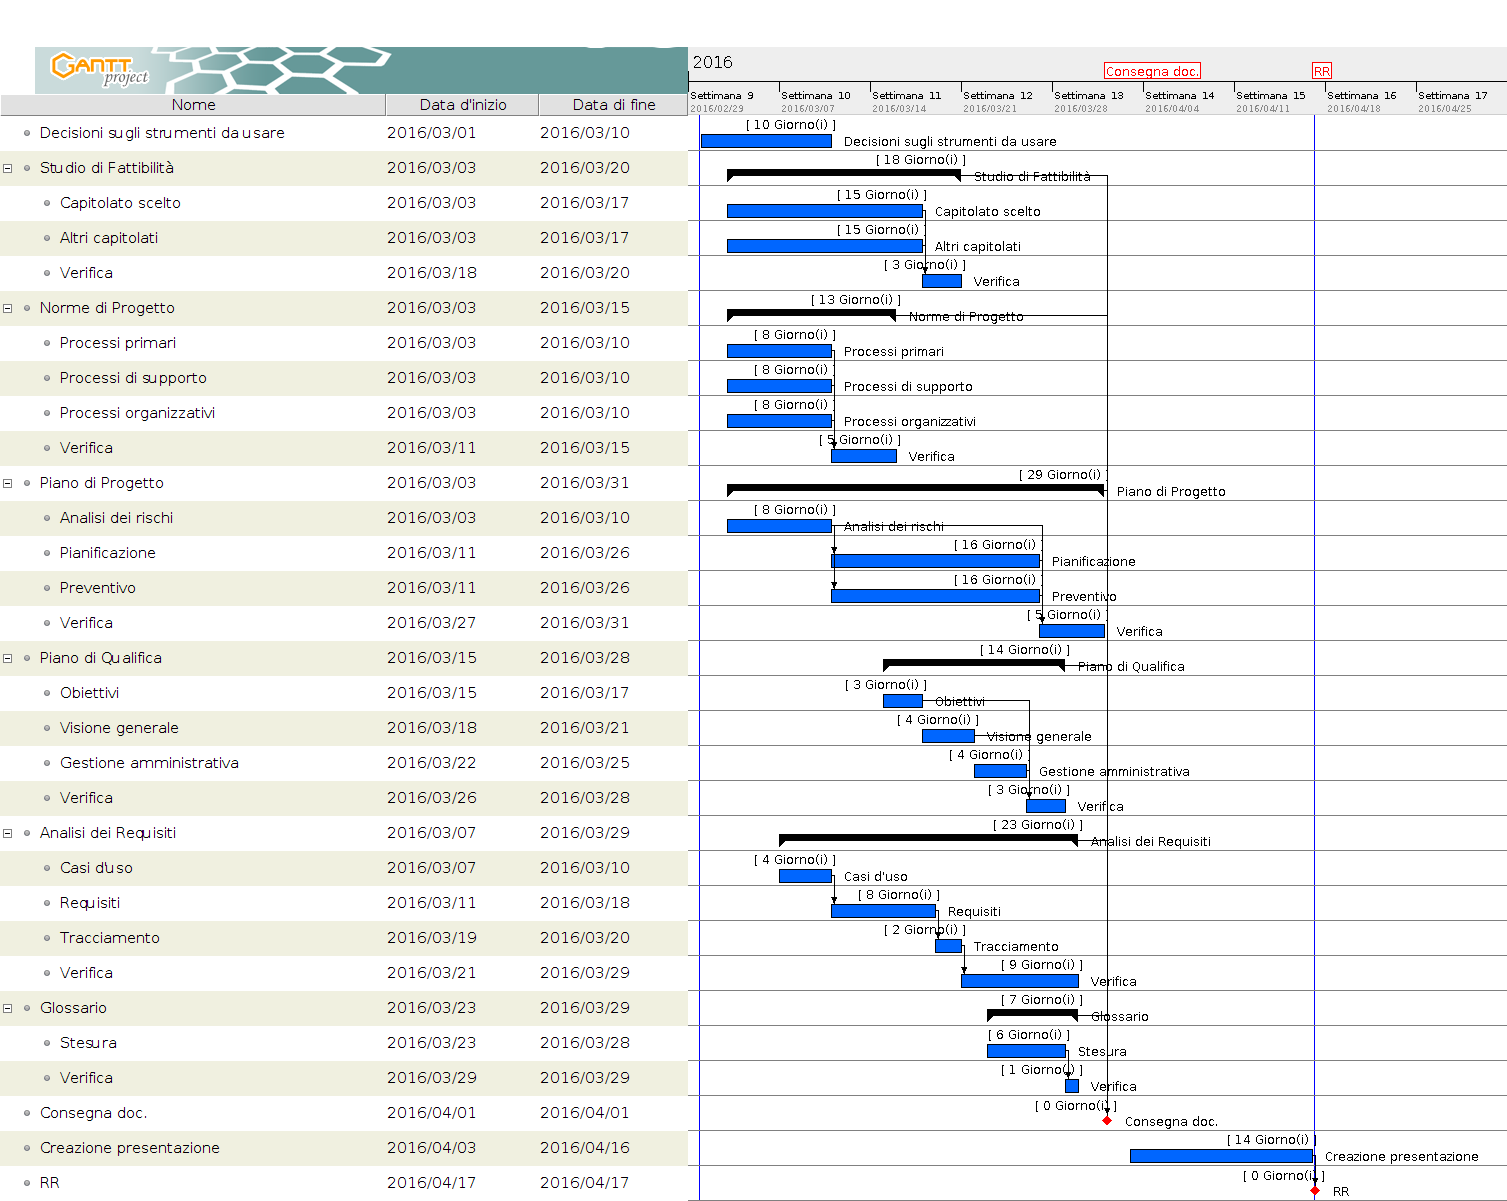
\includegraphics[height=12cm, width=15cm]{img/gantt/A} 
			\caption{Diagramma di Gantt delle attività - Fase A}
		\end{figure}
		
	\subsection{Fase AD}
	\begin{center}
		\textbf{Data di inizio}: 2016/04/19 \\
		\textbf{Data di fine}: 2016/04/28 \\
	\end{center}
	Questa fase inizia al termine della fase A, ovvero dopo la Revisione dei Requisiti, e termina esattamente dieci giorni dopo \\ 
	Il processo principale di questa fase è:
	\begin{itemize}
		\item \textbf{Miglioramento e incremento della documentazione}
		\att
		\begin{itemize}
			\item \textbf{Miglioramento di tutti i documenti}: seguendo le indicazioni del Committente verranno attuate le modifiche necessarie a migliorare tutti i documenti stesi nella fase A;
			\item \textbf{Analisi dei Requisiti}: Questo documento oltre ad essere corretto verrà anche arricchito con nuovi requisiti.
		\end{itemize}
	\end{itemize}
		
		
		\subsubsection{Diagramma di Gantt delle attività}
		\gantt{img/gantt/AD}{Diagramma di Gantt delle attività - Fase AD}
		
	\subsection{Fase PA}
	\begin{center}
		\textbf{Data di inizio}: 2016/04/29 \\
		\textbf{Data di fine}: 2016/06/17 \\
	\end{center}
	Questa fase inizia subito dopo il termine della fase AD e termina con la data della Revisione di Progettazione. \\
	Il processo principale di questa fase è:
		\begin{itemize}
			\item \textbf{Miglioramento e incremento della documentazione}
			\att
			\begin{itemize}
				\item \textbf{Specifica Tecnica}: viene creato il documento \STdoc che conterrà le scelte progettuali decise dai progettisti;
				\item \textbf{Norme di Progetto}: viene incrementato questo documento in modo da normare anche la stesura del documento \STdoc.
				\item \textbf{Piano di Progetto}: viene aggiunto il consuntivi del periodo e preventivo a finire. Vengono inoltre riportati i rischi che si sono verificati nelle fasi precedenti;
				\item \textbf{Piano di Qualifica}: viene aggiunta la parte di pianificazione dei test;
				\item \textbf{Glossario}: viene incrementato con i nuovi termini presenti nella \STdoc.
			\end{itemize}
		\end{itemize}
		\subsubsection{Diagramma di Gantt delle attività}
		\gantt{img/gantt/PA}{Diagramma di Gantt delle attività - Fase PA}
		
		
		
	\subsection{Fase PDC}
	\begin{center}
		\textbf{Data di inizio}: 2016/06/18 \\
		\textbf{Data di fine}: 2016/08/24 \\
	\end{center}
	Questa fase inizia subito dopo la fine della fase PA, ovvero dopo la Revisione di Progettazione, e termina con la data della Revisione di Qualifica. \\
	I processi principali di questa fase sono: 
		\begin{itemize}
			\item \textbf{Miglioramento e incremento della documentazione}
			\att
			\begin{itemize}
				\item \textbf{Definizione di Prodotto}: viene steso il documento \DPdoc il quale definisce la struttura e la relazione tra le componenti del prodotto. È basato sul documento \STdoc;
				\item \textbf{Manuale utente}: viene redatta la versione preliminare del \MUdoc il quale fornirà agli utenti le indicazioni per l'utilizzo del prodotto;
				\item \textbf{Incremento altri documenti}: come nella fase precedente anche in questa vi sarà il miglioramento dei documenti che necessitano tale trattamento.
			\end{itemize}
			\item \textbf{Sviluppo del prodotto}
			\att
			\begin{itemize}
				\item \textbf{Codifica}: avviene la scrittura del codice dei requisiti obbligatori del prodotto;
				\item \textbf{Verifica}: per verificare l'efficacia del codice prodotto nell'attività di codifica vengono eseguiti i test di unità e di integrazione e ne vengono osservati i risultati. 
			\end{itemize}
		\end{itemize}
		\subsubsection{Diagramma di Gantt delle attività}
		% \gantt{img/gantt/PDC}{Diagramma di Gantt delle attività - Fase PDC}
		
		\begin{figure}[!h]
			\centering
			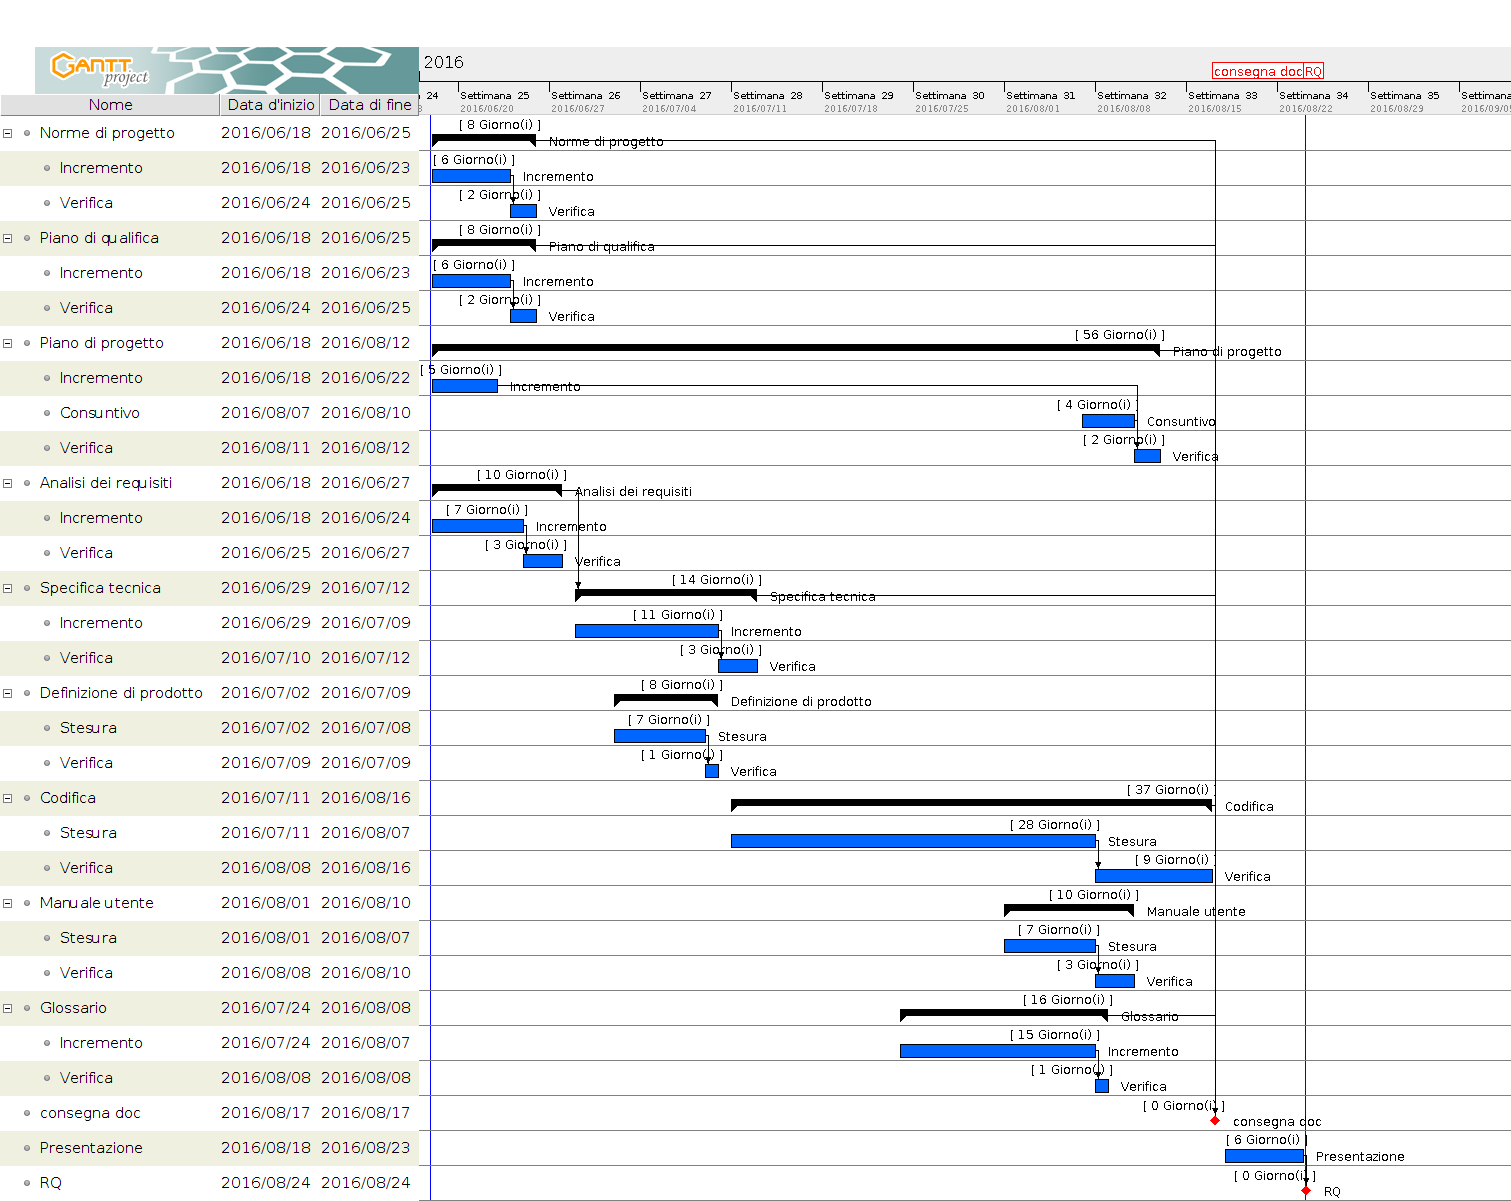
\includegraphics[height=12cm, width=15cm]{img/gantt/PDC} 
			\caption{Diagramma di Gantt delle attività - Fase PDC}
		\end{figure}
		
	\subsection{Fase RD}
	\begin{center}
		\textbf{Data di inizio}: 2016/08/25 \\
		\textbf{Data di fine}: 2016/08/30 \\
	\end{center}
	Questa fase inizia subito dopo la fine della fase PDC, ovvero dopo la Revisione di Qualifica, e termina sei giorni dopo. \\
	I processi principali di questa fase sono: 
		\begin{itemize}
			\item \textbf{Miglioramento e incremento della documentazione}:
			\att
			\begin{itemize}
				\item \textbf{Correzioni e aggiornamenti}: Verranno corretti e aggiornati tutti i documenti che lo necessitano. 
			\end{itemize}
			\item \textbf{Sviluppo del prodotto}:
			\att
			\begin{itemize}
				\item \textbf{Codifica}: avviene la scrittura del codice dei requisiti desiderabili e opzionali del prodotto;
				\item \textbf{Verifica}: per verificare l'efficacia del codice prodotto nell'attività di codifica vengono eseguiti i test di unità e di integrazione e ne vengono osservati i risultati. 
			\end{itemize}
		\end{itemize}
		\subsubsection{Diagramma di Gantt delle attività}
		% \gantt{img/gantt/RD}{Diagramma di Gantt delle attività - Fase RD}
		
		\begin{figure}[!h]
			\centering
			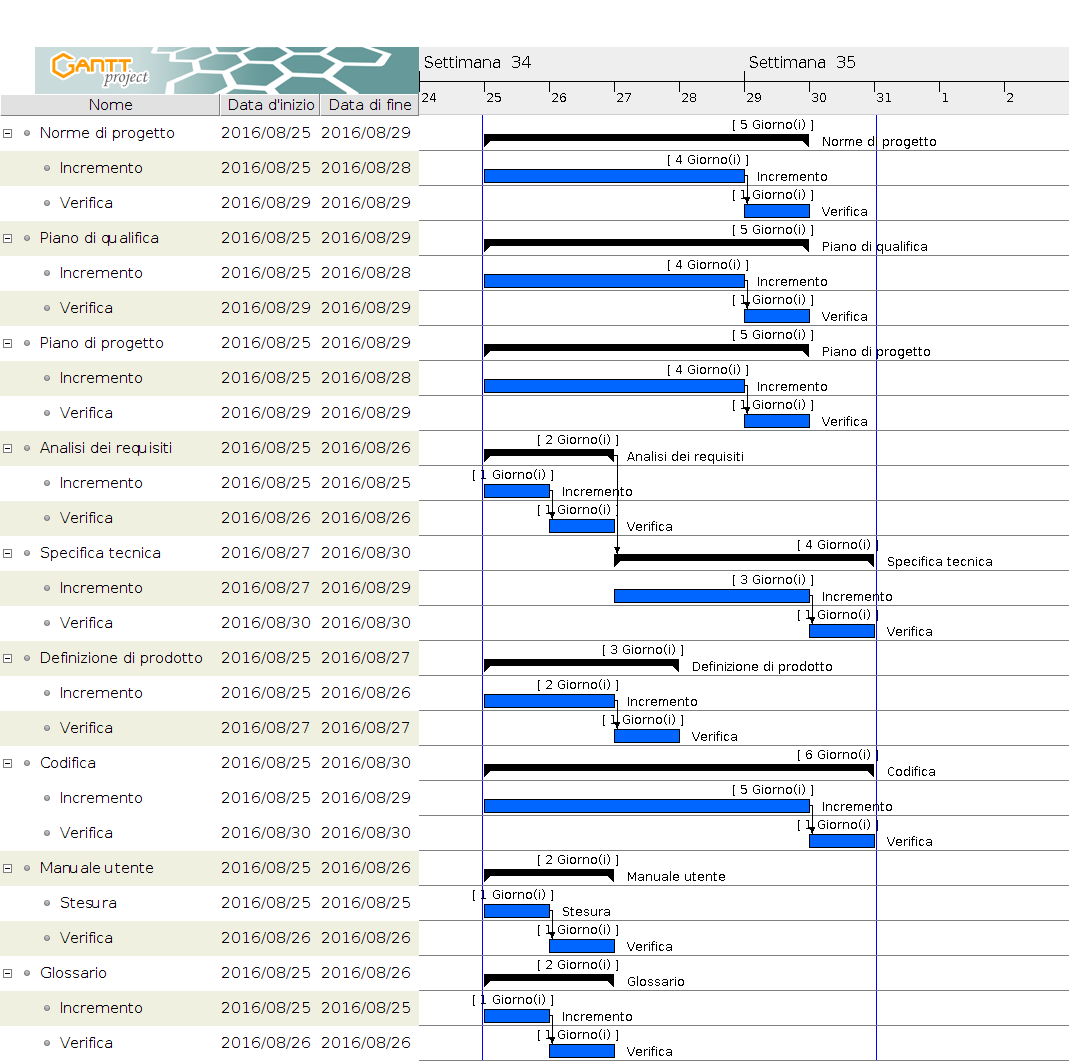
\includegraphics[height=12cm, width=15cm]{img/gantt/RD} 
			\caption{Diagramma di Gantt delle attività - Fase RD}
		\end{figure}
		
	\subsection{Fase V}
	\begin{center}
		\textbf{Data di inizio}: 2016/08/31 \\
		\textbf{Data di fine}: 2016/09/12 \\
	\end{center}
	Questa fase inizia subito dopo la fine della fase RD e termina con la data della Revisione di Accettazione. \\
	I processi principali di questa fase sono:
		\begin{itemize}
			\item \textbf{Miglioramento e incremento della documentazione}
			\att
			\begin{itemize}
				\item \textbf{Correzioni e aggiornamenti}: Verranno corretti e aggiornati tutti i documenti che lo necessitano. Si otterrà la versione finale della documentazione. 
			\end{itemize}
			\item \textbf{Sviluppo del prodotto}
			\att
				\begin{itemize}
					\item \textbf{Test}: vengono eseguiti i test di sistema previsti e ne vengono osservati e monitorati i risultati. 
				\end{itemize}
			\item \textbf{Verifica e validazione}
			\att
			\begin{itemize}
				\item \textbf{Collaudo}: il prodotto viene collaudato sulle funzionalità previste;
				\item \textbf{Verifica}: tramite tracciamento si verifica di aver soddisfatto i requisiti presenti nel documento \ARdoc. Si verificheranno inoltre i canoni di qualità previsti nel \PQdoc;
				\item \textbf{Validazione}: una volta svolte tutte le verifiche il prodotto può considerarsi validato.
			\end{itemize}
		\end{itemize}
		\subsubsection{Diagramma di Gantt delle attività}
		% \gantt{img/gantt/V}{Diagramma di Gantt delle attività - Fase V}
		
		\begin{figure}[!h]
			\centering
			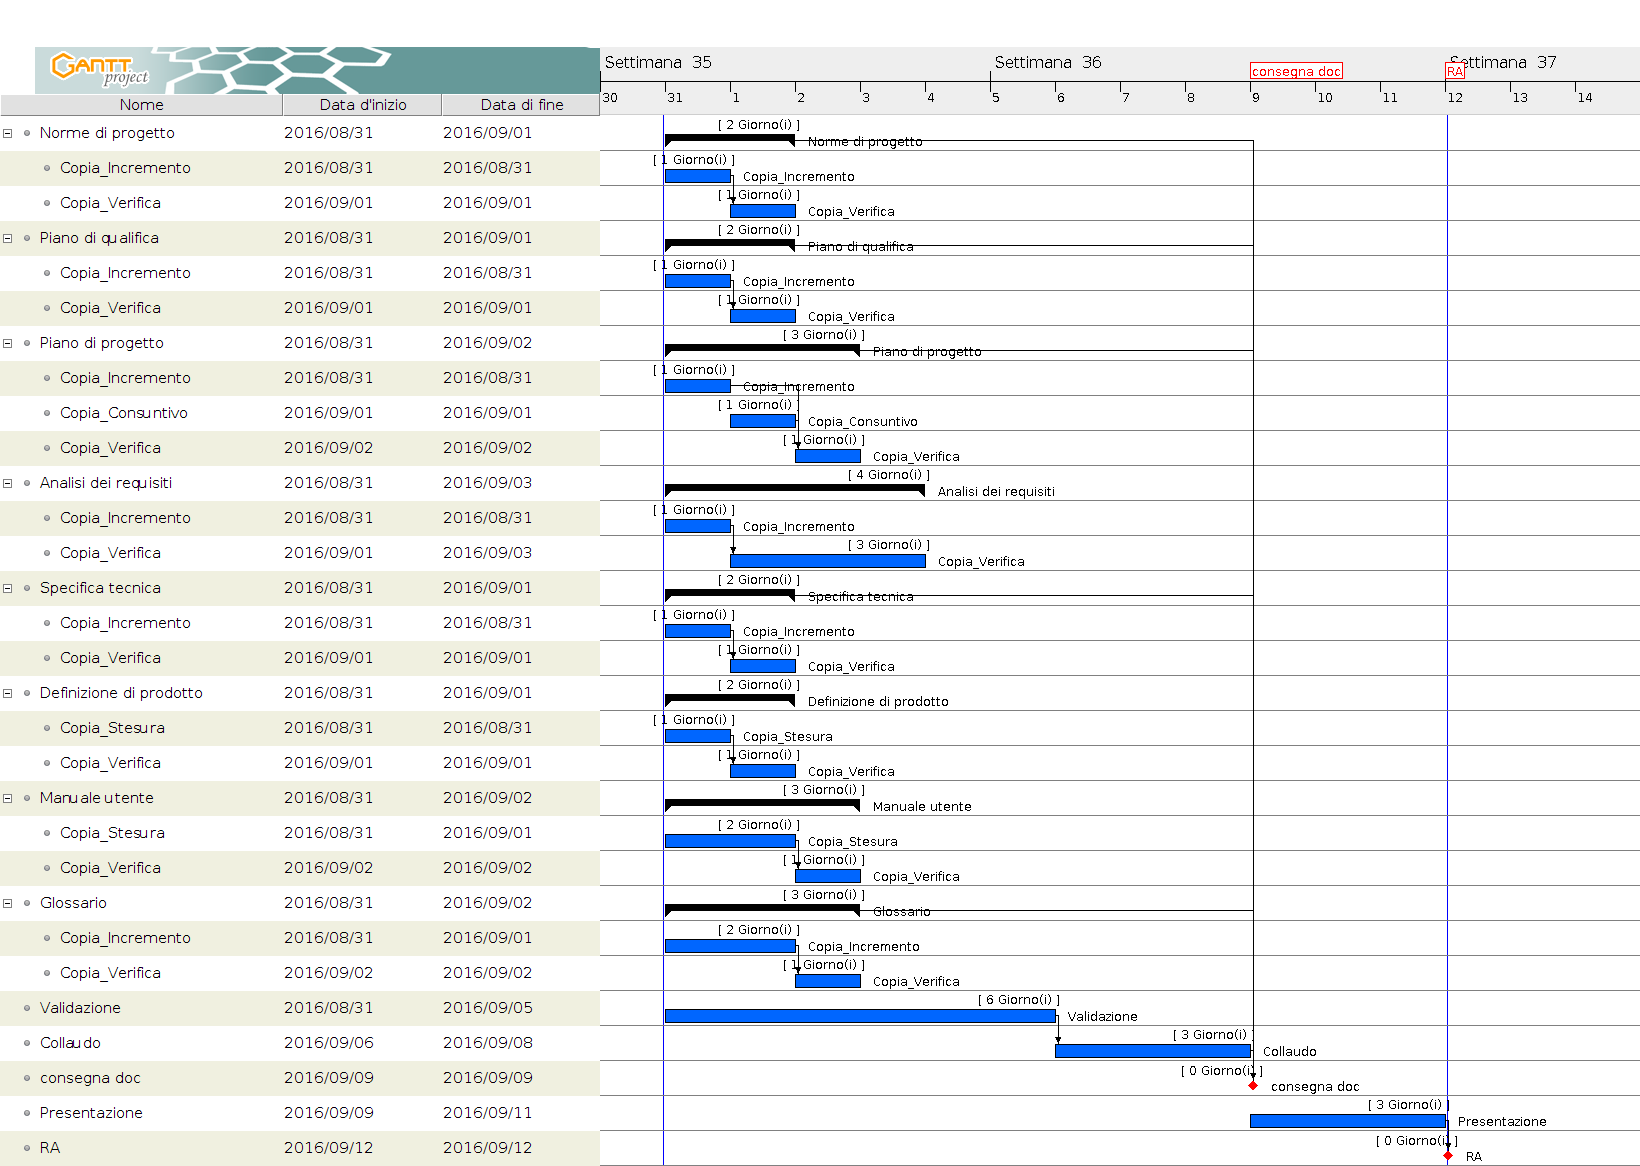
\includegraphics[height=11cm, width=15cm]{img/gantt/V} 
			\caption{Diagramma di Gantt delle attività - Fase V}
		\end{figure}
